\documentclass[10pt]{scrreprt}
\usepackage[utf8]{inputenc}
\usepackage{amsfonts}
\usepackage{amsmath}
\usepackage{amssymb}
\usepackage{commath}
\usepackage[ngerman]{babel}
\usepackage{enumitem}
\usepackage{booktabs}
\usepackage{longtable}
\usepackage{relsize}
\usepackage{pgfplots}
\usepackage{csvsimple}
\usepackage{pgfplotstable}
\usepackage{siunitx}
\usepackage{fancyhdr}
\usepackage{color}
\usepackage{float}
\usepackage{listings}
\usepackage{graphicx}
\usepackage{subcaption}
\usepackage[europeanresistors]{circuitikz}
\usepackage{multirow}
\usepackage{tikz-timing}

\newcommand\tikzmark[1]{%
  \tikz[overlay,remember picture] \coordinate (#1);}

\definecolor{mygreen}{RGB}{28,172,0} % color values Red, Green, Blue
\definecolor{mylilas}{RGB}{170,55,241}


\lstset{language=Matlab,%
%basicstyle=\color{red},
breaklines=true,%
morekeywords={matlab2tikz},
keywordstyle=\color{blue},%
morekeywords=[2]{1}, keywordstyle=[2]{\color{black}},
identifierstyle=\color{black},%
stringstyle=\color{mylilas},
commentstyle=\color{mygreen},%
showstringspaces=false,%without this there will be a symbol in the places where there is a space
%numbers=left,%
%numberstyle={\tiny \color{black}},% size of the numbers
%numbersep=9pt, % this defines how far the numbers are from the text
emph=[1]{for,end,break},emphstyle=[1]\color{red}, %some words to emphasise
%emph=[2]{word1,word2}, emphstyle=[2]{style},
}

\setlength\parindent{0pt}

\setcounter{chapter}{1}
\setcounter{secnumdepth}{2}
\setcounter{section}{0}

\pagestyle{fancy}
\fancyhf{}
\lhead{GPET Versuch 11}
\rhead{Tim Luchterhand, Paul Nykiel}
\cfoot{\thepage}

\author{Tim Luchterhand, Paul Nykiel \protect\\ tim.luchterhand@uni-ulm.de, paul.nykiel@uni-ulm.de}
\title{GPET Versuch 11 --- George Boole - voll integriert!}
\subtitle{Gruppe: Dienstag14}

\begin{document}
    \maketitle
    \chapter{Vorbereitende Aufgaben}
    \section{Vom Halbaddierer zum Volladdierer}
    \begin{enumerate}
        \item
        Skizzieren Sie den Schaltplan des HA in Abbildung~\ref{fig:halbadd} gemäß Wahrheitstabelle.
            \begin{figure}[H]
                \centering
                \begin{circuitikz}\draw
                   (0,0) node[european and port] (and) {}
                   (.3,2) node[european xor port] (xor) {}

                   (xor.in 1) node[left=3cm](x) {x}
                   (and.in 1) node[left=1cm](y) {y}
                   (xor.out) node[above right=1cm](s) {s}
                   (and.out) node[below right=1cm](c) {c}

                   (xor.out) -| (s)
                   (and.out) -| (c)

                   (x) -| (and.in 2)
                   (x) -| (xor.in 1)

                   (y) -| (and.in 1)
                   (y) -| (xor.in 2);
                \end{circuitikz}
                \caption{Halbaddierer}
                \label{fig:halbadd}
            \end{figure}
        \item
            Erweitern Sie die Schaltung zu einem FA und skizzieren Sie sie in Abbildung~\ref{fig:volladdkomp}
            \begin{figure}[H]
                \centering
                \begin{circuitikz} \draw
                    (5,6) node[european xor port] (xyxor) {}
                    (9,6) node[european xor port] (sxor) {}
                    (5,4) node[european and port] (xyand) {}
                    (7,0) node[european and port] (cand) {}
                    (9,2) node[european or port] (cor) {}
                    (0,-1) to[short, l=$X$] (0, 7)
                    (1,-1) to[short, l=$Y$] (1, 7)
                    (2,-1) to[short, l=$C_{in}$] (2, 7)

                    (xyxor.out) -| (sxor.in 1)
                    (xyand.out) -| (cor.in 1)
                    (cand.out) -| (cor.in 2)
                    (xyxor.out) -| (cand.in 1)

                    (0,6.25) to [short, *-] (xyxor.in 1)
                    (1,5.7) to [short, *-] (xyxor.in 2)
                    (7.25,5) to [short, -|] (sxor.in 2)
                    (2,5) to [short, *-] (7.25,5)

                    (0,4.25) to [short, *-] (xyand.in 1)
                    (1,3.7) to [short, *-] (xyand.in 2)

                    (2, -0.3) to [short, *-] (cand.in 2)

                    (sxor) node [above right=1cm](s) {$S$}
                    (cor) node [below right=1cm](c) {$C$}

                    (sxor.out) -| (s)
                    (cor) -| (c)
                ;\end{circuitikz}
                \caption{Komplizierter Volladdier}
                \label{fig:volladdkomp}
            \end{figure}
        \item
            Versuchen Sie die FA-Schaltung so umzuformen, dass Ihnen zwei Quad-Gatter
            genugen. Notieren Sie die Herleitung und zeichnen Sie die Schaltung in Abbildung~\ref{fig:volladdeinf}.

            Mithilfe der De-Morganschen-Identität ergibt sich:
            \begin{equation*}
                a + b = \overline{\overline{a+b}} = \overline{\overline{a} \cdot \overline{b}}
            \end{equation*}
            \begin{figure}[H]
                \centering
                \begin{circuitikz} \draw
                    (5,6) node[european xor port] (xyxor) {}
                    (9,6) node[european xor port] (sxor) {}
                    (5,4) node[european nand port] (xyand) {}
                    (7,0) node[european nand port] (cand) {}
                    (9,2) node[european nand port] (cor) {}
                    (0,-1) to[short, l=$X$] (0, 7)
                    (1,-1) to[short, l=$Y$] (1, 7)
                    (2,-1) to[short, l=$C_{in}$] (2, 7)

                    (xyxor.out) -| (sxor.in 1)
                    (xyand.out) -| (cor.in 1)
                    (cand.out) -| (cor.in 2)
                    (xyxor.out) -| (cand.in 1)

                    (0,6.25) to [short, *-] (xyxor.in 1)
                    (1,5.7) to [short, *-] (xyxor.in 2)
                    (7.25,5) to [short, -|] (sxor.in 2)
                    (2,5) to [short, *-] (7.25,5)

                    (0,4.25) to [short, *-] (xyand.in 1)
                    (1,3.7) to [short, *-] (xyand.in 2)

                    (2, -0.3) to [short, *-] (cand.in 2)

                    (sxor) node [above right=1cm](s) {$S$}
                    (cor) node [below right=1cm](c) {$C$}

                    (sxor.out) -| (s)
                    (cor) -| (c)
                ;\end{circuitikz}
                \caption{Vereinfachter Volladdier}
                \label{fig:volladdeinf}
            \end{figure}
    \end{enumerate}

    \section{Schaltungsdefekte}
    Die folgenden Fragen sollen sicherstellen, dass Sie die theoretischen Vorraussetzungen
    erfüllen, um den Versuch durchführen zu können, der sich mit Stuck-at-0/1-Problemen
    befasst.
    \begin{enumerate}
        \item Welche zwei Schritte sind nötig um einen Knoten zu testen - und wie ergibt sich
            daraus der Testvektor?

            Will man einen bestimmten Knoten K des Netzes auf einen Stuck-at-Fehler prüfen,
            so müssen zwei Schritte durchgeführt werden. Durch eine geeignete Beschaltung der
            Eingänge muss zum einen sichergestellt werden, dass der Zustand des zu beobachtenden
            Knotens am Ausgang sichtbar wird; d.h.\ die nachfolgenden Gatter müssen so beschal-
            tet sein, dass sie transparent werden, also den ankommenden, zu beobachtenden Pegel
            weitergeben. Anschließend muss der zu testende Knoten noch eingestellt werden.
            Will man prüfen, ob sich ein Knoten fest auf einer 0 befindet (stuck-at-0), muss er
            testhalber auf 1 gesetzt werden --- und umgekehrt. Ergibt sich bei diesem Einstellvektor
            kein Widerspruch zum Beobachtungsvektor, kann die Schnittmenge beider Vektoren als
            Testvektor verwendet werden.
        \item Sind auf diese Weise alle Fehler detektierbar?

            Nein:
            \begin{itemize}
                \item bei mehreren Fehlern kann der defekte Knoten nicht eindeutig bestimmt werden
                \item zum Teil können die folgenden Gatter nicht transparent geschalten werden, da sie ebenfalls von den Eingängen abhängen
            \end{itemize}
        \item Wie können folgende Gatter für einen ihrer Eingänge mit Belegung \glqq{}D\grqq{} transparent
            geschaltet werden und wie verhält sich dann der Ausgang?
            \begin{table}[H]
                \centering
                \begin{tabular}{c|c|c|c}
                    \toprule
                    Gatter & $IN_1$ & $IN_{2 \ldots N}$ & OUT\\
                    \midrule
                    AND & D & 1 & D\\
                    NAND & D & 1 & $\overline{\text{D}}$\\
                    OR & D & 0 & D\\
                    NOR & D & 0 & $\overline{\text{D}}$\\
                    XOR & D & 0 & D\\
                    \bottomrule
                \end{tabular}
                \caption{Beschaltung einzelner Gattereingänge für Transparenz}
            \end{table}
    \end{enumerate}

    \section{Hazards und Glitches}
    Wesentliche Limitationen von Schaltnetzen sind die endlichen Laufzeiten von Gattern.
    Nicht nur, dass durch sie die Geschwindigkeit der Berechnung einer Booleschen Funk-
    tion begrenzt wird; Gatterlaufzeiten können auch zu Instabilitäten von Schaltnetzen
    führen. Dabei ist ein Hazard die Eigenschaft eines Schaltnetzes, mögliche Instabilitäten
    zu beinhalten. Das konkrete Auftreten einer Instabilität ist z.B. ein Glitch. Das heißt,
    das während der Laufzeit der Signale kurzzeitig ein falsches Zwischenergebnis an den
    Ausgängen anliegt und sich ein Spannungswert ändert, obwohl dies laut der Booleschen
    Funktion nicht der Fall wäre.

    \begin{enumerate}
        \item Stellen Sie ein KV-Diagramm in Abbildung~\ref{fig:hazzard} für die Boolesche Funktion aus
            Tabelle 12a auf und geben Sie die minimierte Funktion an.

            \begin{table}[H]
                \centering
                \begin{tabular}{cc|cccc}
                    & &  & \multicolumn{2}{c}{yz}\\
                    & & 10 & 11 & 01 & 00\\
                    \midrule
                    \multirow{ 2}{*}{x} & 1 & 1 & 1 & 1 & 0\\
                     & 0 & 0 & 0 & 1 & 0\\
                \end{tabular}
                \caption{KV-Diagramm eines Hazard-behafteten Schaltnetzes}
                \label{fig:hazzard}
            \end{table}
            \begin{equation*}
                o(x,y,z) = x \cdot y + \overline{y} \cdot z
            \end{equation*}
        \item Zeichnen Sie einen Schaltplan dieser Funktion mit AND-, OR- und NOT-Gattern
            in den dafur vorgesehenen Platz in Abbildung~\ref{fig:schaltungGlitch}.

            \begin{figure}[H]
                \centering
                \begin{circuitikz} \draw
                    (4,0) node[european not port] (ynot) {}
                    (6,2) node[european and port] (yzand) {}
                    (6,6) node[european and port] (xyand) {}
                    (8,4) node[european or port] (finalor) {}
                    (0,-1) to[short, l=$X$] (0, 7)
                    (1,-1) to[short, l=$Y$] (1, 7)
                    (2,-1) to[short, l=$Z$] (2, 7)

                    (finalor.out) node [above right=1cm](o) {$o$}

                    (ynot.out) -| (yzand.in 2)
                    (yzand.out) -| (finalor.in 2)
                    (xyand.out) -| (finalor.in 1)
                    (finalor.out) -| (o)


                    (1,0) to [short, *-] (ynot.in)
                    (2,2.25) to [short, *-] (yzand.in 1)
                    (1,5.7) to [short, *-] (xyand.in 2)
                    (0,6.25) to [short, *-] (xyand.in 1)
                ;\end{circuitikz}
                \caption{Zeichnen Sie hier Schaltung ein, die der ermittelten Normalform des
        Glitch-behafteten Schaltnetzes entspricht}
                \label{fig:schaltungGlitch}
            \end{figure}
        \item Vervollständigen Sie das Timing-Diagramm in Abbildung~\ref{fig:timeGlitch}. Dabei soll eine Einheit
            in der Horizontalen der Laufzeit eines Gatters entsprechen.

            \begin{figure}[H]
                \centering
                \begin{tikztimingtable}
                    [timing/slope=0,timing/coldist=2pt,
                    xscale=2.5,yscale=2]
                    x & 19H \\
                    y & 3H 8L 8H\\
                    z & 19H \\
                    xy & 4H 8L 7H\\
                    $\overline{\text{y}}$ & 4L 8H 7L\\
                    z$\overline{\text{y}}$ & 5L 8H 6L\\
                    o & 4H 1L 14H\\
                    \extracode
                    \tablegrid[black!25]
                    \draw[red, thick] (4.5,-11.5) circle(.25cm);
                \end{tikztimingtable}
                \caption{Timing Diagramm einer digitalen Schaltung}
                \label{fig:timeGlitch}
            \end{figure}
        \item Identifizieren und markieren Sie den Glitch. Erläutern Sie, durch welchen Umstand
            es zum Glitch in $o$ kommt.

            Durch die Unterschiedlich \glqq{}langen\grqq{} Pfade in der Schaltung
            verschieben sich die Signale zeitlich zueinander. Dadurch kommt es
            zu einem Glitch am Ausgang.
    \end{enumerate}

    \setcounter{chapter}{3}
    \chapter{Versuchsdurchführung}
    \section{Volladdierer}
    Zunächst sollen Sie mit der Aufteilung des PCB-Boards vertraut werden und den Umgang
    mit den Laborkabeln anhand eines einfachen Beispiels verinnerlichen.
    \begin{enumerate}
        \item Bauen Sie einen Volladdierer gemäß Ihrer Vorbereitung auf. Realisieren Sie die
            Variante, die nur zwei Logikbausteine erfordert.
        \item Verifizieren Sie die Wahrheitstabelle und zeigen Sie den Aufbau Ihrem Betreuer.
    \end{enumerate}

    \paragraph{Protokoll}
    Der aufgebaute Volladierer funtioniert, wie erwartet, ordnungsgemäß.

    \section{Ermittlung der Logikfunktion}
    Beginnen Sie zunächst damit, die Ihnen unbekannte Schaltung A in Bereich (E) zu
    untersuchen.
    \begin{enumerate}
        \item Erstellen Sie die Wahrheitstabelle der unbekannten Funktion.
        \item Ermitteln Sie mit Hilfe eines KV-Diagramms die minimierte Normalform der
            Schaltung. Lassen Sie Ihr Ergebnis durch Ihren Tutor überprüfen. Sie können sich nun
            die Schaltung in der Black-Box ansehen und Ihre Lösung verifizieren.
    \end{enumerate}

    \paragraph{Protokoll}
    $ $
    \begin{table}[H]
        \centering
        \begin{tabular}{cccc|c}
            \toprule
            a & b & c & d & out \\
            \midrule
            0 & 0 & 0 & 0 & 0\\
            1 & 0 & 0 & 0 & 1\\
            0 & 1 & 0 & 0 & 1\\
            1 & 1 & 0 & 0 & 0\\
            0 & 0 & 1 & 0 & 0\\
            1 & 0 & 1 & 0 & 1\\
            0 & 1 & 1 & 0 & 1\\
            1 & 1 & 1 & 0 & 0\\
            0 & 0 & 0 & 1 & 0\\
            1 & 0 & 0 & 1 & 1\\
            0 & 1 & 0 & 1 & 1\\
            1 & 1 & 0 & 1 & 0\\
            0 & 0 & 1 & 1 & 0\\
            1 & 0 & 1 & 1 & 1\\
            0 & 1 & 1 & 1 & 0\\
            1 & 1 & 1 & 1 & 0\\
            \bottomrule
        \end{tabular}
        \caption{Wahrheitstabelle der Schaltung A}
    \end{table}

    Minimierte Normalform:
    \begin{eqnarray*}
        \text{out} &=& a\cdot \bar{b} + \bar{a} \cdot \bar{d} \cdot b + b \cdot \bar{a} \cdot \bar{c}\\
            &=& a \cdot \bar{b} + \bar{a} \cdot b \cdot (\bar{c} + \bar{d})
    \end{eqnarray*}

    Die Schaltung in der Blackbox stimmt mit der Normalform überein.

    \begin{table}
        \centering
        \begin{tabular}{cc|cccc}
            & &  & \multicolumn{2}{c}{BD}\\
            & & 10 & 11 & 01 & 00\\
            \midrule
             & 10 & 0 & 0 & 1 & 1\\
            \multirow{ 2}{*}{AC} & 11 & 0 & 0 & 1 & 1\\
             & 01 & 1 & 0 & 0 & 0\\
             & 00 & 1 & 1 & 0 & 0
        \end{tabular}
        \caption{KV-Diagramm}
    \end{table}


    \section{Aufspüren eines Schaltungsdefektes}
    Die zweite Schaltung (B) ist identisch zur soeben untersuchten, jedoch weicht ihr Verhal-
    ten auf Grund eines Defektes ab. Ein Knoten des Schaltnetzes ist stets auf konstantem
    Potenzial, unabhängig von der Belegung der Eingänge (stuck-at-0/1-Problem). Im Fol-
    genden sollen Sie Art und Ort des Defektes bestimmen.
    \begin{enumerate}
        \item Erstellen Sie auch für dieses Schaltnetz die Wahrheitstabelle (Sch.B).
        \item Welcher Baustein auf dem \textit{DigiBoard} eignet sich, um auf den ersten Blick
            Unterschiede im Verhalten der beiden Schaltungen zu erkennen?
        \item Nutzen Sie einen solchen Baustein um die Unterschiede des Verhaltens der beiden
            Schaltungen zu ermitteln und stellen Sie diese in einer Tabelle (Differenz) dar.
        \item Betrachten Sie nur die Knoten $K_1$ - $K_3$. Finden Sie geeignete Testvektoren, um
            etwaige Defekte aufzuspüren:
        \item Ermitteln Sie Ort und Art des Defektes.
    \end{enumerate}

    \paragraph{Protokoll}
    $ $
    \begin{table}[H]
        \centering
        \begin{tabular}{cccc|c}
            \toprule
            a & b & c & d & out \\
            \midrule
            0 & 0 & 0 & 0 & 0\\
            1 & 0 & 0 & 0 & 0\\
            0 & 1 & 0 & 0 & 1\\
            1 & 1 & 0 & 0 & 0\\
            0 & 0 & 1 & 0 & 0\\
            1 & 0 & 1 & 0 & 0\\
            0 & 1 & 1 & 0 & 1\\
            1 & 1 & 1 & 0 & 0\\
            0 & 0 & 0 & 1 & 0\\
            1 & 0 & 0 & 1 & 0\\
            0 & 1 & 0 & 1 & 1\\
            1 & 1 & 0 & 1 & 0\\
            0 & 0 & 1 & 1 & 0\\
            1 & 0 & 1 & 1 & 0\\
            0 & 1 & 1 & 1 & 0\\
            1 & 1 & 1 & 1 & 0\\
            \bottomrule
        \end{tabular}
        \caption{Wahrheitstabelle für Schaltung B}
    \end{table}
    Man schaltet die Ausgänge der beiden Schaltungen mit einem XOR zusammen. Sobald
    die Ausgänge nicht identisch sind, ist der Ausgang des XORs auf high und sonst
    auf low.
    \begin{table}[H]
        \centering
        \begin{tabular}{cccc|cc}
            \toprule
            a & b & c & d & $out_a$ & $out_b$\\
            \midrule
            1 & 0 & 0 & 0 & 1 & 0\\
            1 & 0 & 0 & 1 & 1 & 0\\
            1 & 0 & 1 & 0 & 1 & 0\\
            1 & 0 & 1 & 1 & 1 & 0\\
            \bottomrule
        \end{tabular}
        \caption{Differenz der beiden Schatungen}
    \end{table}

    \subparagraph{Testvektoren}
    \begin{eqnarray*}
        &K_1:& \overline{a} \cdot \overline{b} \cdot c \cdot d,\ \overline{a} \cdot b \cdot c \cdot d,\ a \cdot \overline{b} \cdot c \cdot d,\ a \cdot b \cdot c \cdot d\\
        &K_2:& \overline{a} \cdot \overline{b} \cdot \overline{cd},\ a \cdot \overline{b} \cdot \overline{cd},\ \overline{a} \cdot b \cdot \overline{cd},\ a \cdot b \cdot \overline{cd}\\
        &K_3:& \overline{a} \cdot b \cdot \overline{c} \cdot \overline{d},\ \overline{a} \cdot b \cdot c \cdot \overline{d},\ \overline{a} \cdot b \cdot \overline{c} \cdot d,\ \overline{a} \cdot b \cdot c \cdot d
    \end{eqnarray*}

    \begin{table}[H]
        \centering
        \begin{tabular}{cc|c}
            \toprule
            a & b & $K_1$\\
            \midrule
            0 & 0 & 0\\
            0 & 1 & 0\\
            1 & 0 & 0\\
            1 & 1 & 0\\
            \bottomrule
        \end{tabular}
        \caption{Testvektor bei $K_1$}
    \end{table}

    Aus dieser Tabelle erkennt man, dass der Knoten $K_1$ immer auf 0V liegt, also
    ein \glqq Stuck-at-0\grqq~bei $K_1$.

    \section{Doppel-XOR}
    \begin{figure}[H]
        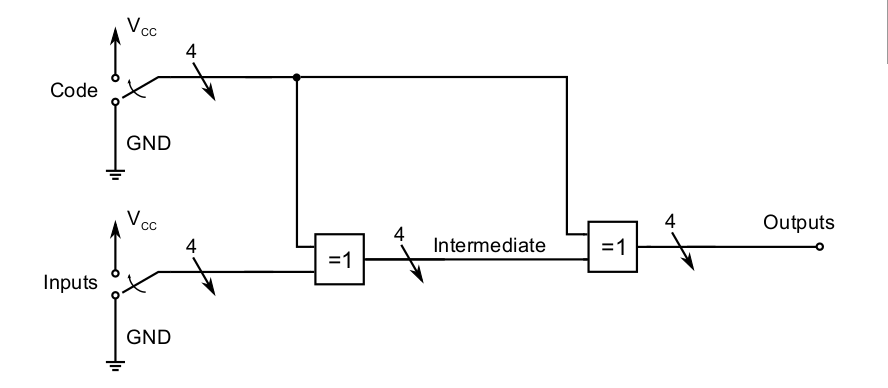
\includegraphics[width=\textwidth]{abb14.png}
        \caption{Versuch mit Doppel-XOR}
        \label{fig:abb14}
    \end{figure}
    Bauen Sie zunächst eine Schaltung aus 2 Quad-XORs gemäß Abbildung~\ref{fig:abb14} auf. Die
    mit 4 gekennzeichneten Pfeile stehen für einen Bus mit vier Adern, das heißt, die dort
    gezeigte Schaltung ist vier mal parallel aufzubauen. Verwenden Sie sowohl für die vier
    \textit{Inputs} als auch für die vier \textit{Code}-Eingänge jeweils vier zusammenhängende Schalter aus
    Bereich (B), mit denen Sie zwischen \textit{GND} und $V_{DD}$ wechseln können. Wenn Sie die vier
    \textit{Intermediate}-Signale und die vier \textit{Outputs} auf die LED-Bank in Bereich (G) legen, können
    Sie die Zustände gut vergleichen. Es bietet sich an, die vier zusammengehörenden Signale
    jeweils auf eine Reihe der LED-Bank zu geben und die selbe Reihenfolge zu nutzen.
    Stellen Sie nun eine beliebige aber konstante Eingangskombination für die vier \textit{Inputs}
    ein.
    \begin{enumerate}
        \item Welcher Effekt lässt sich an den Ausgängen (\textit{Intermediate} und \textit{Output}) beobachten,
            wenn Sie bei konstanten \textit{Input}-Eingängen eine andere Kombinationen auf die \textit{Code}-
            Eingänge geben?
        \item Welcher Effekt lässt sich an den Ausgängen (\textit{Intermediate} und \textit{Output}) beobachten,
            wenn Sie nun nur die \textit{Input}-Eingänge variieren?
        \item Wie lässt sich dieser Effekt mit Hilfe der Booleschen Gleichungen ausdrücken und
            belegen? Zeigen Sie, dass $a \oplus b \oplus b = a$ gilt.
        \item Wofür könnte die Schaltung genutzt werden?
    \end{enumerate}

    \paragraph{Protokoll}
    $ $
    Der eingang Input wir unverändert zum Ausgang Output durchgereicht, der eingang
    Code verändert Output nicht. Am Ausgang Intermediate wird das \glqq{}verschlüsselte\grqq
    ~Eingangssignal ausgegeben.

    Das Verhalten der Schaltung lässt sich durch folgenden boolschen Ausdruck
    beschreiben:

    \begin{equation*}
        a \oplus b \oplus b = a \oplus (b \oplus b)
        = a \oplus 0 = a
    \end{equation*}

    Ohne den Zustand des Codeeingangs zu kennen, lässt sich nur mit Kenntnis des
    Intermediate-Ausgangs nicht der eigentliche Eingangszustand bestimmen. Es handelt
    sich also um eine einfache Verschlüsselung.

    \section{Verwendung der digitalen Oszilloskop-Eingänge}
    Einführend sollen Sie die Gatterlaufzeiten eines AND, NOR, NOT und eines XOR
    ermitteln. Hierfür werden Sie die digitalen Eingänge des Oszilloskops verwenden.

    \subsection{Bereitstellung geeigneter Eingangssignale}
    Sie können mit Hilfe des Taster \textit{CLK} aus Bereich (C) eine entprellte Flanke erzeugen.
    Verwenden Sie auf jeden Fall nur diesen Taster, da die anderen Schalter nicht entprellt
    sind und die Messung dadurch verfälscht werden könnte. Die benachoverlinete LED zeigt den
    aktuellen Pegel an. Sie benötigen zusätzlich zwei Jumper; mit dem Einen verbinden Sie
    den \textit{CLK}-Taster mit der \textit{CLK}-Leitung, mit dem Zweiten verbinden Sie in Bereich (F)
    eine der Buchsen mit der \textit{CLK}-Leitung. Anschließend können Sie an dieser Buchse die
    Flanke abgreifen. Führen Sie dieses Signal sowohl auf einen Eingang des zu vermessenden
    Gatters, als auch auf einen \textit{Output} in Bereich (G), sodass Sie am Oszilloskop auf die
    Flanke triggern können. Abbildung~\ref{fig:abb15} verdeutlicht die benötigten Schritte nochmals.
    Beschalten Sie den zweiten Eingang des zu vermessenden Gatter so, dass die erzeugte
    Flanke zu einem Zustandswechsel führt.
    \begin{figure}[H]
        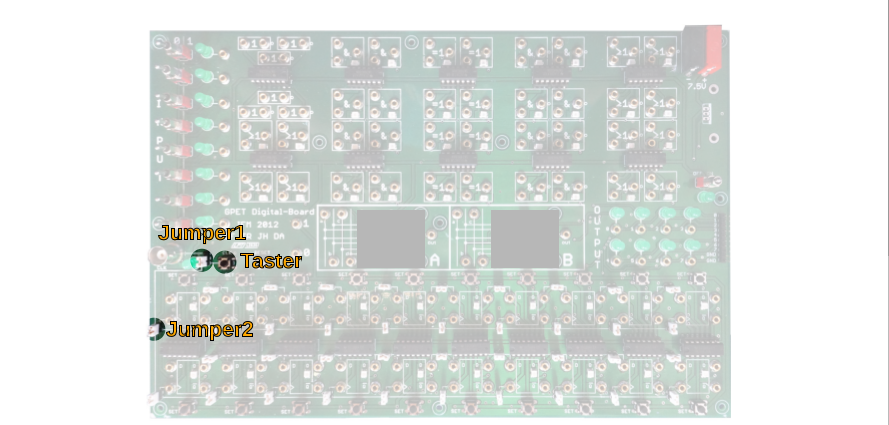
\includegraphics[width=\textwidth]{abb15.png}
        \caption{Abgreifen einer entprellten Flanke}
        \label{fig:abb15}
    \end{figure}

    \subsection{Einstellungen am Oszilloskop}
    Verbinden Sie auf Seiten des \textit{DigiBoards} die Kabelpeitsche mit der Pin-Leiste in Bereich
    (G) und achten Sie dabei auf die Beschriftung der einzelnen Kabel. Das Ende mit dem
    Flachbandkabel kann an der Frontseite des Oszilloskops eingesteckt werden. Setzen Sie
    das Oszilloskop mittels \framebox{Default Setup} zurück und deaktivieren Sie die analogen Kanäle
    1 und 2. Per \framebox{Digital} gelangen Sie in das Menü zur Konfiguration der digitalen Eingänge.
    Mit den kontextabhängigen Knöpfen unterhalb des Displays wählen sie zunächst die richtige
    Schwellwerteinstellung für CMOS-Gatter (0V-5V, Schwelle ist 2,5V). Sie können nun
    zur Erhöhung der Übersichtlichkeit die Amplitude der Darstellung im Display anpassen
    und nur die benötigten Digital-Eingänge anwählen. Im \framebox{Trigger}-Menü können Sie schließ-
    lich den digitalen Eingang auswählen, der die Flanke liefert. Führen Sie dann die entspre-
    chenden Messungen als Einzelmessung über \framebox{Single} durch. Ermitteln Sie die Laufzeiten
    für die Gatter AND, NOR, NOT und XOR.

    \paragraph{Protokoll}
    \begin{figure}[H]
        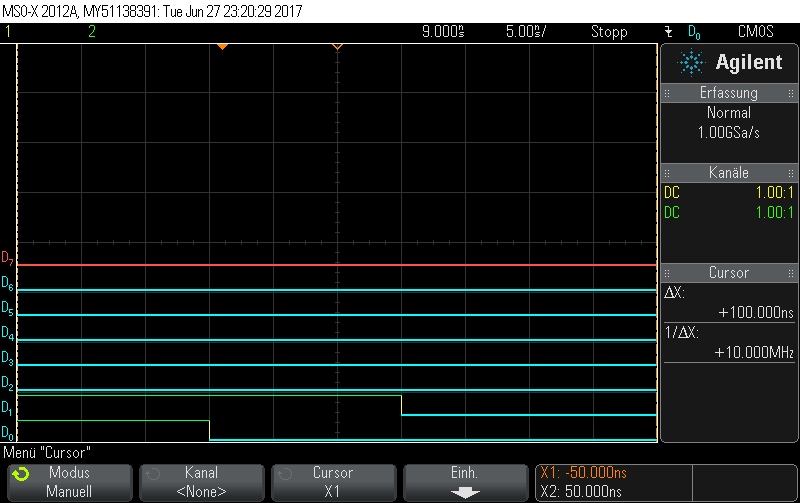
\includegraphics[width=\textwidth]{scope_8.png}
        \caption{Laufzeit für das AND-Gatter}
    \end{figure}

    Laufzeit: $15\si{n\second}$

    \begin{figure}[H]
        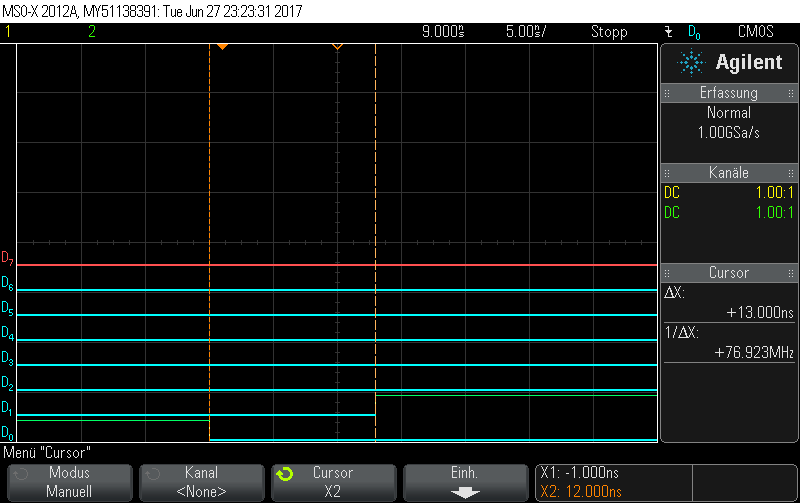
\includegraphics[width=\textwidth]{scope_9.png}
        \caption{Laufzeit für das NOR-Gatter}
    \end{figure}

    Laufzeit: $13\si{n\second}$

    \begin{figure}[H]
        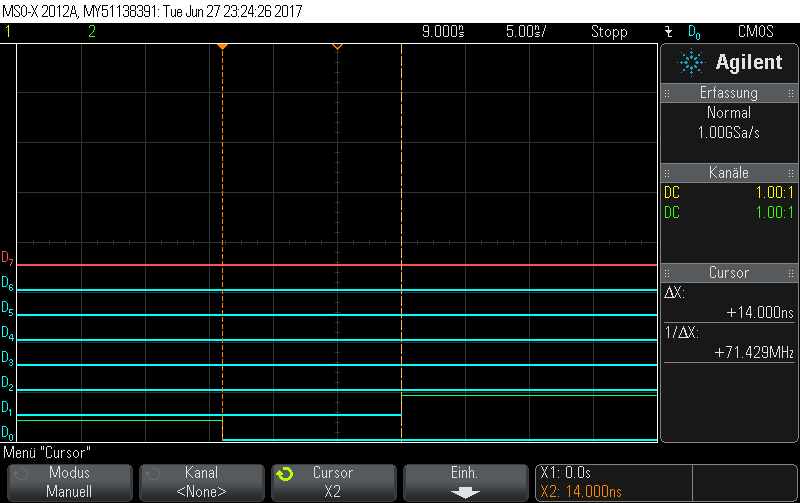
\includegraphics[width=\textwidth]{scope_10.png}
        \caption{Laufzeit für das NOT-Gatter}
    \end{figure}

    Laufzeit: $14\si{n\second}$

    \begin{figure}[H]
        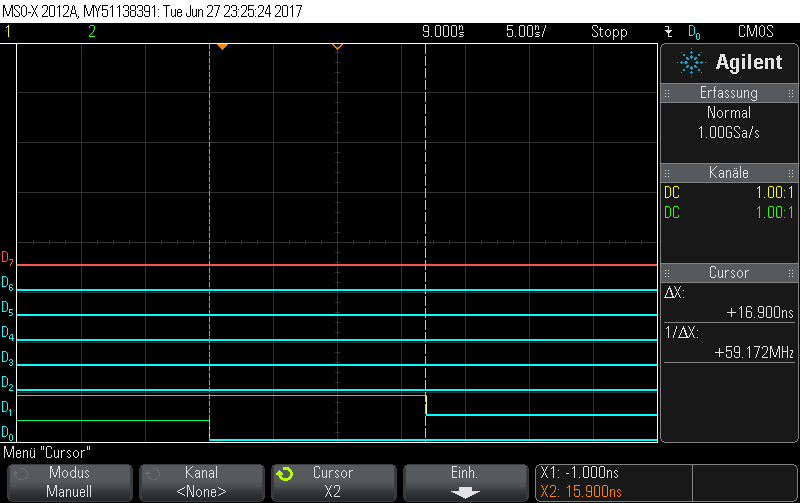
\includegraphics[width=\textwidth]{scope_11.png}
        \caption{Laufzeit für das XOR-Gatter}
    \end{figure}

    Laufzeit: $17\si{n\second}$

    \section{Zeitverhalten der Gattersignale}
    \begin{figure}[H]
        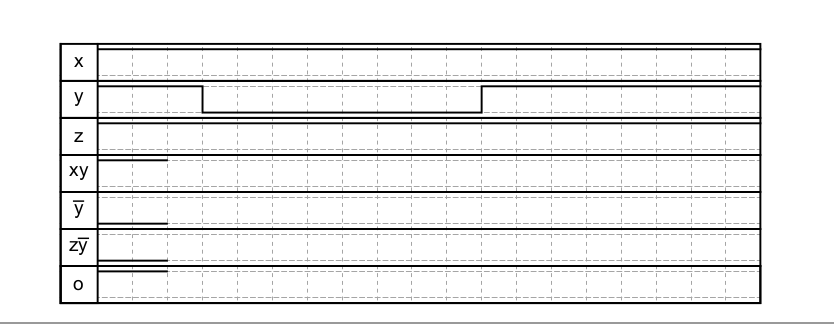
\includegraphics[width=\textwidth]{abb13.png}
        \caption{Timing Diagramm einer digitalen Schaltung}
        \label{fig:abb13}
    \end{figure}
    Wir wollen den Glitch aus der Vorbereitungsaufgabe nachvollziehen.
    \begin{enumerate}
        \item Bauen Sie die Schaltung gemäß der Vorbereitungsfrage auf und verifizieren Sie die
            Wahrheitstabelle.
        \item Wählen Sie für $x$ den Kanal 7 und führen sie alle weiteren Signale gemäß Abbildung
            \ref{fig:abb13} auf die weiteren Ausgänge ($x \rightarrow 7 \ldots o \rightarrow 1$). Dadurch lässt sich die Ausbreitung
            der Signale innerhalb der Schaltung gut beobachten.
            Wir wollen nun das Timing-Diagramm nachmessen. Hierfür setzen Sie $x = z = 1$
            und erzeugen mit Hilfe des \textit{CLK}-Tasters eine fallende Flanke auf $y$. Am Ozilloskop
            triggern Sie nun auf den Kanal, der die fallende Flanke von y führt. Stellen Sie am
            Oszilloskop eine geeignete zeitliche Auflösung ein, um sowohl die fallende Flanke
            als auch den Glitch sehen zu können. Messen Sie alle Signale der Schaltung und
            fügen Sie einen screenshot in Ihr Protokoll ein. Lassen Sie die Schaltung für den
            folgenden Versuch aufgebaut.
            \subsubsection{Hinweis}
            Sollten Sie den Glitch nicht sehen obwohl sich die Schaltung ansonsten erwartungsgemäß verhält,
            versuchen Sie andere UND-Gatter zu verwenden. Durch Toleranzen
            der Bauteillaufzeiten kann es im \glqq{}ungünstigsten\grqq{} Fall passieren, dass der Glitch
            zufällig unterdrückt wird.
    \end{enumerate}

    \paragraph{Protokoll}
    $ $
    \begin{figure}[H]
        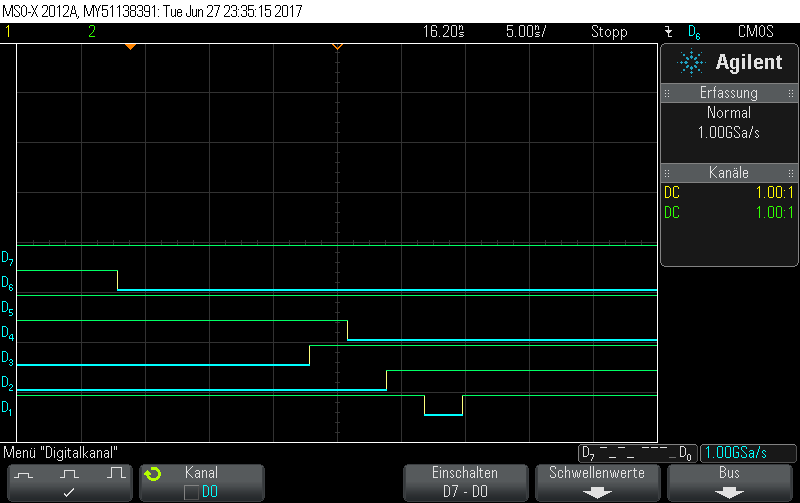
\includegraphics[width=\textwidth]{scope_12.png}
        \caption{Auftretender Glitch}
    \end{figure}

    Der Glitch ist in Form eines kurzen Low-Pegels beim Eingang $D_1$ deutlich
    zu sehen.

    \section{Gegenmaßnahmen bei Glitches}
    Der gemessene Glitch ist eine Folge der absoluten Minimierung der Normalform. Glitches
    können immer auftreten, wenn im KV-Diagramm keine Überdeckungen zwischen den
    Termen bestehen. Im Rückschluss können Hazards vermieden werden, indem man durch
    Hinzufügen von Termen zusätzliche Überdeckungen schafft. Die Funktion ist dann nicht
    mehr minimal, aber frei von Hazards.

    \begin{enumerate}
        \item Stellen Sie erneut ein KV-Diagramm auf. Das Schaltnetz soll jedoch durch Hin-
            zufügen eines Terms immun gegen den beobachteten Glitch werden. Heben Sie den
            Term hervor, der eine Überdeckung der beiden bisherigen Einkreisungen herstellt.
            Wie muss die Hazard-freie Funktion lauten?
        \item Zeichnen Sie den Schaltplan der neuen Funktion auf Gatter-Ebene und zeigen Sie
            diesen Ihrem Tutor.
        \item Erweitern Sie Ihre Schaltung auf dem \textit{DigiBoard} gemäß dem Schaltplan und legen
            das neue Ausgangssignal auf den letzten verbleibenden Digital-Eingang.
        \item Messen Sie das Timing-Diagramm für die fallende Flanke von $y$ wie im vorhergehenden
            Versuch und diskutieren Sie, ob und wie das Einfügen des zusätzlichen Terms
            den Glitch verhindert.
    \end{enumerate}

    \paragraph{Protokoll}
    $ $

    \begin{table}[H]
        \centering
        \begin{tabular}{cc|cccc}
            & &  & \multicolumn{2}{c}{yz}\\
            & & 10 & 11 & 01 & 00\\
            \midrule
            \multirow{ 2}{*}{x} & 1 & \textcolor{red}{1} & \underline{\textcolor{red}{1}} & \underline{\textcolor{blue}{1}} & 0\\
             & 0 & 0 & 0 & \textcolor{blue}{1} & 0\\
        \end{tabular}
        \caption{KV-Diagramm}
    \end{table}

    Daraus ergibt sich die Normalform:
    \begin{equation*}
        \text{out} = x \cdot y + z \cdot \bar{y} + \mathbf{x \cdot z}
    \end{equation*}

    \begin{figure}[H]
        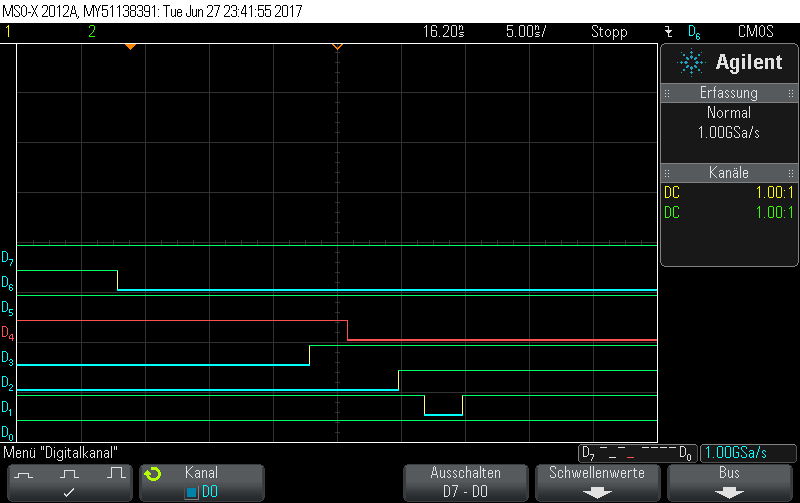
\includegraphics[width=\textwidth]{scope_13.png}
        \caption{Glitch tritt nicht mehr auf}
    \end{figure}

    \begin{figure}[H]
        \centering
        \begin{circuitikz} \draw
        (0,3) node[european and port] (xyand) {}
        (7,2) node[european or port] (finalor) {}
        (5,1) node[european or port] (bottomor) {}
        (3,2) node[european and port] (xzand) {}
        (3,0) node[european and port] (yzand) {}
        (0,0) node[european not port] (ynot) {}


        (xyand.in 1) node[above left=1cm](x) {x}
        (xyand.in 2) node[below left=1cm](y) {y}
        (y) node[below=.5cm](z){z}

        (xyand.out) -| (finalor.in 1)
        (bottomor.out) -| (finalor.in 2)

        (yzand.out) -| (bottomor.in 2)
        (xzand.out) -| (bottomor.in 1)

        (x) -| (xzand.in 1)
        (z) -| (xzand.in 2)

        (y) -| (ynot.in)

        (ynot.out) -| (yzand.in 2)
        (z) -| (yzand.in 1)

        (x) -| (xyand.in 1)
        (y) -| (xyand.in 2);

        \end{circuitikz}
        \caption{Schaltung ohne Glitch}
        \label{}
    \end{figure}




    Wie in der überarbeiteten Schaltung zu erkennen, wird das glitchbehaftete Signal
    nun zusätzlich mit $x \cdot z$ verodert. Dadurch verschwindet der kurze Low-Pegel.

\end{document}
